\documentclass[11pt]{article}
\usepackage[margin=0.9in]{geometry}
\usepackage{amsmath,amssymb,amsthm}
\usepackage{graphicx}
\usepackage[colorlinks=true,linkcolor=blue,urlcolor=blue,citecolor=blue]{hyperref}
\usepackage{microtype}

\newtheorem{theorem}{Theorem}
\newcommand{\VN}{\mathrm{VN}}
\newcommand{\PG}{\mathcal P_G}
\newcommand{\wstar}{\mathrm{w}^*}

\title{Weak-* closability of the Fourier gradient without the approximation property}
\author{Candidate full solution to Remark 3.13 of arXiv:1903.10151}
\date{11 August 2026}

\begin{document}
\maketitle

\noindent\textbf{Status.}
\texttt{candidate full solution (likely valid; human review requested)}.

\section*{Source problem}
Arhancet and Kriegler \cite{AK} define, for a discrete group $G$, a real
one-cocycle $b_\psi:G\to H$, and $-1\le q<1$, the Fourier gradient
\[
 \partial_{\psi,q}:\PG\subseteq\VN(G)
 \longrightarrow \Gamma_q(H)\rtimes_\alpha G,
 \qquad
 \partial_{\psi,q}(\lambda_s)
   =s_q(b_\psi(s))\rtimes\lambda_s.
\]
Their Proposition~3.12 (PDF pages 53--54) proves weak-* closability when $G$
has the approximation property (AP).  Remark~3.13 (PDF page 54) states:
``We do not know if the assumption `AP' in Proposition 3.12 is really
necessary.''  The result below removes AP completely.

\section*{Transcription of the question}
Is the AP assumption in Proposition~3.12 necessary for weak-* closability of
$\partial_{\psi,q}$?

\clearpage
\section*{Source evidence}
\noindent\textbf{Proposition 3.12 and its weak-* closability definition
(source PDF page 53).}
\begin{center}
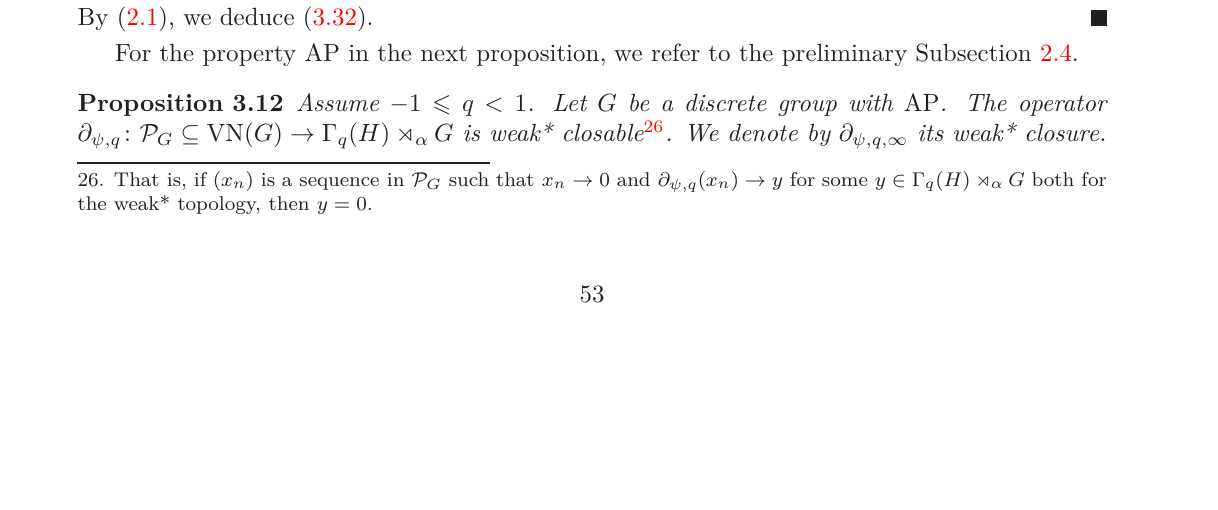
\includegraphics[width=\textwidth]
{figures/open_problem_context_page53.png}
\end{center}

\medskip
\noindent\textbf{End of the source proof and Remark 3.13
(source PDF page 54).}
\begin{center}
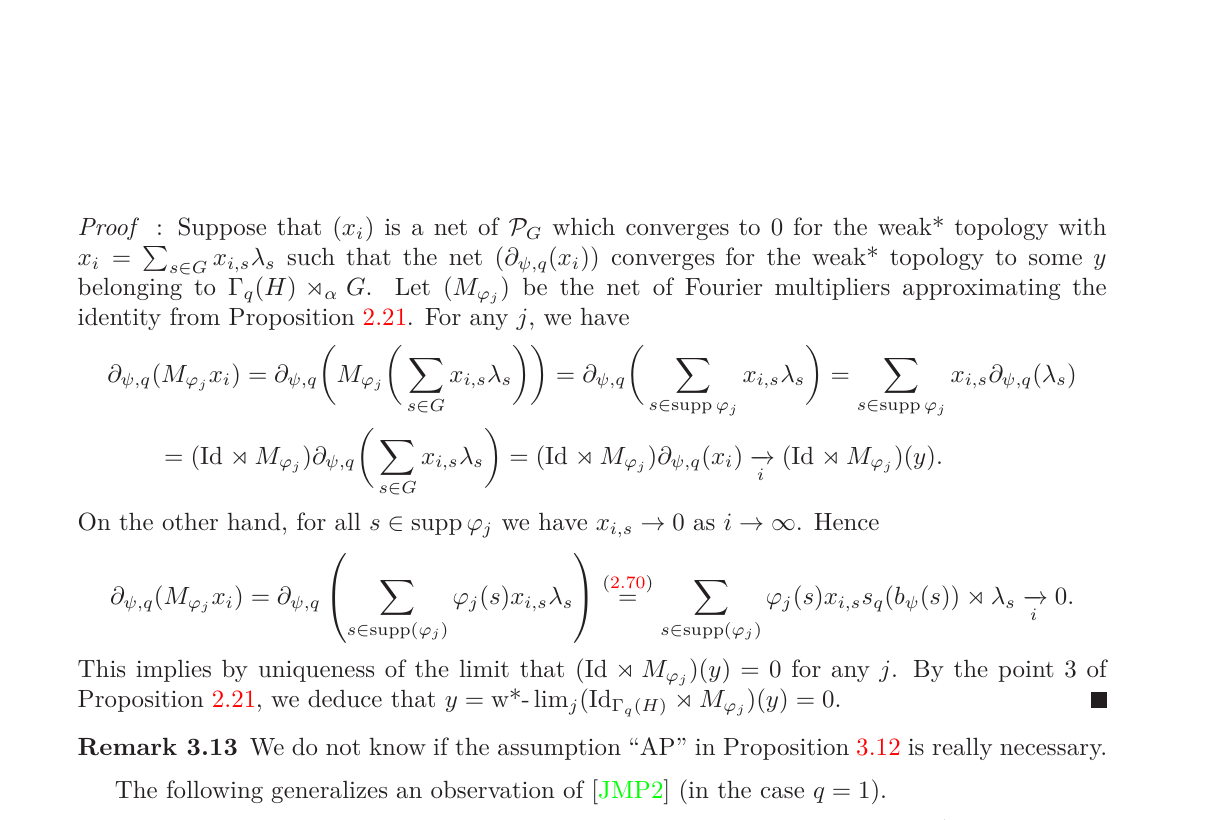
\includegraphics[width=\textwidth]
{figures/open_problem_remark_page54.png}
\end{center}

\clearpage
\section*{Proof intuition}
The gradient is diagonal in the group Fourier variable.  Instead of using AP
to approximate a possible weak-* limit by finite-support multipliers, extract
each crossed-product Fourier coefficient directly.  Coefficient extraction is
normal, every coefficient of a graph limit above zero vanishes, and the
orthogonal Fourier decomposition of the crossed-product $L^2$ space makes the
coefficients separating.

\begin{theorem}
Let $G$ be any discrete group, let $b_\psi:G\to H$ and $\alpha$ be as in the
source construction, and let $-1\le q<1$.  Then
\[
 \partial_{\psi,q}:\PG\subseteq\VN(G)
 \longrightarrow \Gamma_q(H)\rtimes_\alpha G
\]
is weak-* closable.  In particular, AP is unnecessary in
Proposition~3.12 of \cite{AK}.
\end{theorem}

\begin{proof}
Put $N=\Gamma_q(H)\rtimes_\alpha G$, and let
$E_\Gamma:N\to\Gamma_q(H)$ be the canonical normal faithful conditional
expectation.  For $s\in G$, define the Fourier coefficient map
\[
 C_s:N\longrightarrow\Gamma_q(H),
 \qquad C_s(z)=E_\Gamma\bigl(z(1\rtimes\lambda_s)^*\bigr).
\]
It is weak-* continuous because $E_\Gamma$ and right multiplication by a fixed
unitary are normal.  On Fourier polynomials,
\[
 C_s\left(\sum_{t\in F}a_t\rtimes\lambda_t\right)=a_s.
\]

Suppose that a net $(x_i)$ in $\PG$ satisfies
\[
 x_i\xrightarrow{\wstar}0,
 \qquad
 \partial_{\psi,q}(x_i)\xrightarrow{\wstar}y\in N.
\]
Write $x_i=\sum_t x_{i,t}\lambda_t$, where each sum is finite.  For every
fixed $s\in G$,
\[
 x_{i,s}=\tau_G(x_i\lambda_s^*)\longrightarrow0,
\]
since $x\mapsto\tau_G(x\lambda_s^*)$ is a normal functional on $\VN(G)$.
The definition of the gradient gives
\[
 C_s\bigl(\partial_{\psi,q}(x_i)\bigr)
 =x_{i,s}s_q(b_\psi(s)).
\]
By normality of $C_s$,
\[
 C_s(y)=\lim_i x_{i,s}s_q(b_\psi(s))=0
 \qquad(s\in G).
\]

Finally, crossed-product Fourier coefficients are unique.  More explicitly,
for the canonical finite trace,
\[
 L^2(N)=\bigoplus_{s\in G}^{\perp}
 L^2(\Gamma_q(H))(1\rtimes\lambda_s),
\]
and $C_s(y)$ is the $s$-th coordinate of $y$.  Since the bounded element
$y\in N$ lies in $L^2(N)$ and all its coordinates vanish, $y=0$.  This is
weak-* closability.  The argument works for nets and therefore also for the
sequential formulation in footnote 26 of \cite{AK}.
\end{proof}

\section*{Verification and limitations}
The only structural inputs are the normal canonical expectation, the explicit
gradient formula, and uniqueness of Fourier coefficients.  The coefficient
convention has been checked directly on $a\rtimes\lambda_t$.  No convergence
of the full Fourier series in operator norm is assumed.  The range
$-1\le q<1$ is retained: at $q=1$ the classical Gaussian field operator is
generally unbounded, so this is not the same von-Neumann-algebra-valued map.
The theorem resolves Remark~3.13 only; it does not address the later endpoint
Lipschitz-algebra or optimal commutator questions.

\section*{Novelty check}
A bounded search on 11 August 2026 covered the run indexes, the exact remark
sentence and label, the source title and arXiv id, combinations of
``weak-* closable'', ``$\Gamma_q$'', ``crossed product gradient'', and ``AP'',
citing-paper results, and the public record of the authors' 2022 Springer
Lecture Notes volume.  No later resolution of Remark~3.13 was found.  This
supports but does not establish novelty.

\section*{Human-review recommendation}
Verify the convention for $C_s$ and the standard orthogonal $L^2$ Fourier
decomposition.  Once those two points are confirmed, the proof has no further
dependency.

\begin{thebibliography}{9}
\bibitem{AK}
C.~Arhancet and C.~Kriegler,
\emph{Riesz transforms, Hodge--Dirac operators and functional calculus for
multipliers I}, arXiv:1903.10151v9 (2020), Remark~3.13;
\href{https://arxiv.org/abs/1903.10151}{arXiv:1903.10151}.
\end{thebibliography}

\end{document}
